\subsection{Allievi}
\subsubsection{Panoramica allievo}

\begin{figure}[H]
\centering
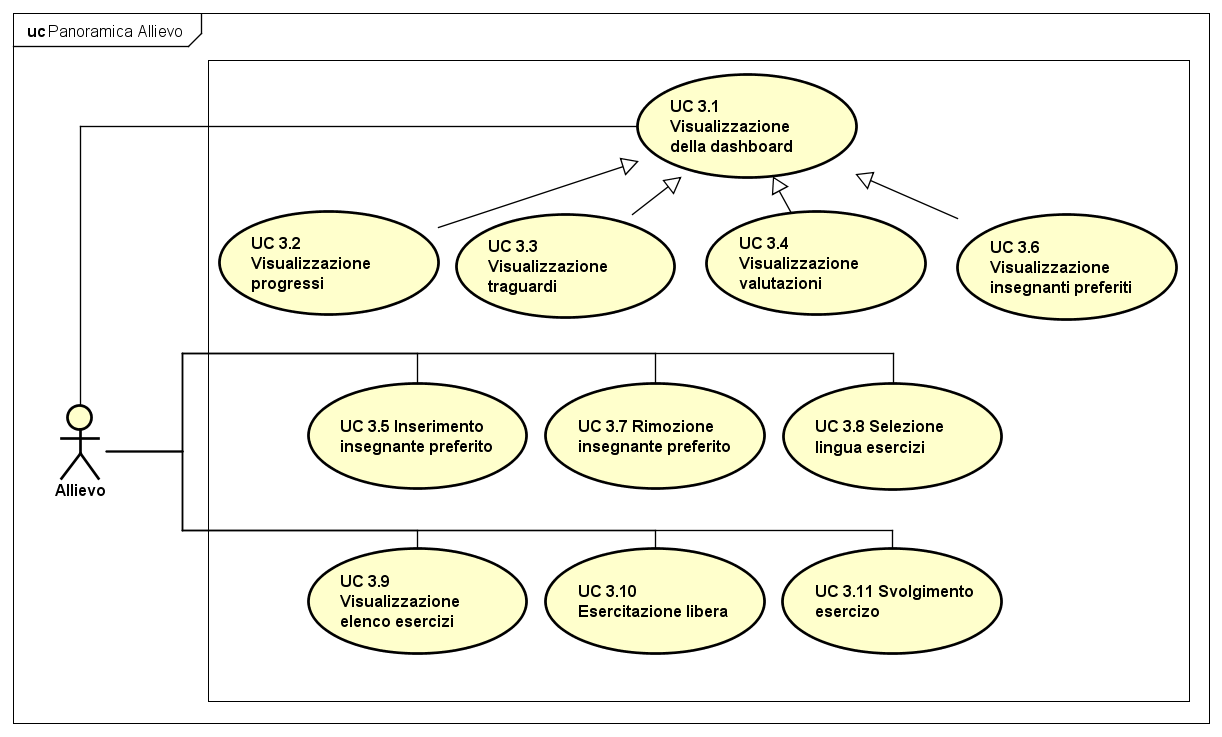
\includegraphics[width=17cm]{img/PanoramicaAllievi.png} 
\caption{Panoramica allievo}\label{fig:31}
\end{figure}


\subsubsection{UC 3.1 - Visualizzazione della dashboard}
\begin{itemize}
\item[•]\textbf{Attori}: Allievo;
\item[•]\textbf{Descrizione}: l'allievo visualizza la propria dashboard;
\item[•]\textbf{Precondizione}: l'allievo si è autenticato;
\item[•]\textbf{Postcondizione}: l'allievo visualizza la dashboard.
\end{itemize}

\subsubsection{UC 3.2 - Visualizzazione progressi}
\begin{itemize}
\item[•]\textbf{Attori}: Allievo;
\item[•]\textbf{Descrizione}: l'allievo visualizza i suoi progressi: numero di esercizi svolti, corretti ed errati;
\item[•]\textbf{Precondizione}: l'allievo visualizza la propria dashboard;
\item[•]\textbf{Postcondizione}: l'allievo visualizza i propri progressi;
\item[•]\textbf{Generalizzazioni}:
\begin{itemize}
\item UC 3.1 - Visualizzazione della dashboard.
\end{itemize}
\end{itemize}
\subsubsection{UC 3.3 - Visualizzazione traguardi}
\begin{itemize}
\item[•]\textbf{Attori}: Allievo;
\item[•]\textbf{Descrizione}: l'allievo visualizza i traguardi raggiunti;
\item[•]\textbf{Precondizione}: l'allievo visualizza la propria dashboard;
\item[•]\textbf{Postcondizione}: l'allievo visualizza tutti i traguardi raggiunti.
\item[•]\textbf{Generalizzazioni}:
\begin{itemize}
\item UC 3.1 - Visualizzazione della dashboard.
\end{itemize}
\end{itemize}

\subsubsection{UC 3.4 - Visualizzazione valutazioni}
\begin{itemize}
\item[•]\textbf{Attori}: Allievo;
\item[•]\textbf{Descrizione}: l'allievo visualizza le valutazioni di tutti gli esercizi svolti, sia esercizi assegnati che svolti indipendentemente;
\item[•]\textbf{Precondizione}: l'allievo visualizza la propria dashboard;
\item[•]\textbf{Postcondizione}: l'allievo visualizza tutte le valutazioni ricevute.
\item[•]\textbf{Generalizzazioni}:
\begin{itemize}
\item UC 3.1 - Visualizzazione della dashboard.
\end{itemize}
\end{itemize}

\subsubsection{UC 3.5 - Inserimento insegnante preferito}
\begin{itemize}
\item[•]\textbf{Attori}: Allievo;
\item[•]\textbf{Descrizione}: l'allievo inserisce il nome utente di un insegnante da prediligere quando riceve la correzione di un esercizio;
\item[•]\textbf{Precondizione}: l'allievo visualizza la propria dashboard;
\item[•]\textbf{Postcondizione}: l'allievo ha inserito un insegnante preferito.
\end{itemize}

\subsubsection{UC 3.6 - Visualizzazione insegnanti preferiti}
\begin{itemize}
	\item[•]\textbf{Attori}: Allievo;
	\item[•]\textbf{Descrizione}: l'allievo visualizza la lista degli insegnanti preferiti che ha inserito;
	\item[•]\textbf{Precondizione}: l'allievo visualizza la propria dashboard;
	\item[•]\textbf{Postcondizione}: l'allievo visualizza gli insegnanti preferiti.
	\item[•]\textbf{Generalizzazioni}:
\begin{itemize}
\item UC 3.1 - Visualizzazione della dashboard.
\end{itemize}
\end{itemize}

\subsubsection{UC 3.7 - Rimozione insegnante preferito}
\begin{itemize}
	\item[•]\textbf{Attori}: Allievo;
	\item[•]\textbf{Descrizione}: l'allievo seleziona dalla lista visualizzata un insegnante da rimuovere dagli insegnanti preferiti;
	\item[•]\textbf{Precondizione}: l'allievo visualizza la lista di insegnanti preferiti;
	\item[•]\textbf{Postcondizione}: l'allievo ha rimosso un insegnante preferito dalla lista.
\end{itemize}

\subsubsection{UC 3.8 - Selezione lingua esercizi}
\begin{itemize}
	\item[•]\textbf{Attori}: Allievo;
	\item[•]\textbf{Descrizione}: l'allievo seleziona la lingua in cui vuole svolgere gli esercizi e visualizzare le soluzioni;
	\item[•]\textbf{Precondizione}: l'allievo visualizza la propria dashboard;
	\item[•]\textbf{Postcondizione}: l'allievo ha selezionato una lingua per gli esercizi.
\end{itemize}

\subsubsection{UC 3.9 - Visualizzazione elenco esercizi}
\begin{itemize}
\item[•]\textbf{Attori}: Allievo;
\item[•]\textbf{Descrizione}: l'allievo visualizza un elenco di frasi consigliate dal sistema come esercizi oppure gli esercizi assegnati dall'insegnante;
\item[•]\textbf{Precondizione}: l'allievo visualizza la propria dashboard;
\item[•]\textbf{Postcondizione}: l'allievo visualizza un elenco di esercizi.
\end{itemize}

\subsubsection{UC 3.10 - Esercitazione libera}
\begin{figure}[H]
	\centering
	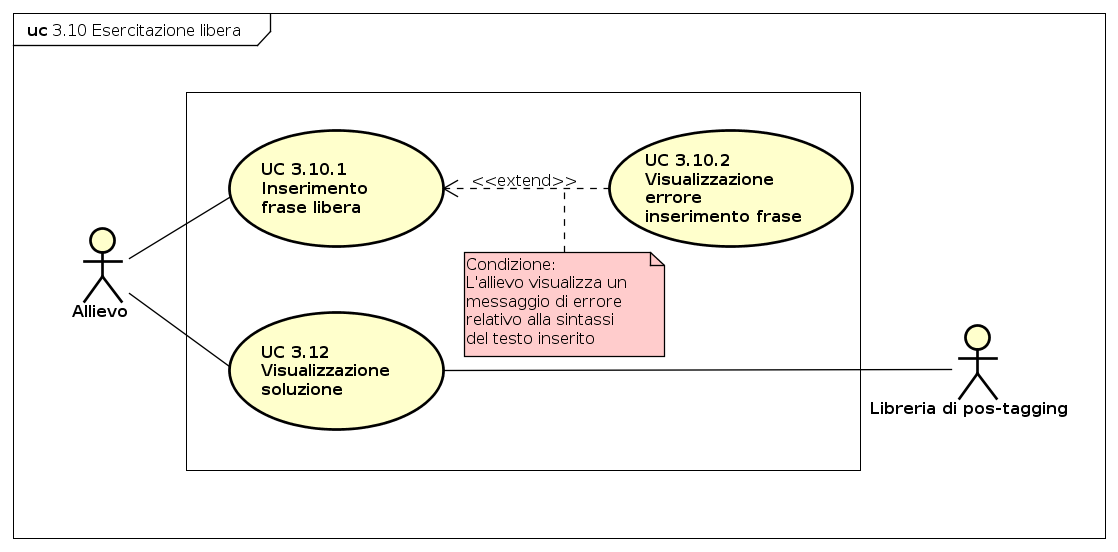
\includegraphics[width=17cm]{img/UC310.png} 
	\caption{Caso d'uso 3.10}\label{fig:310}
\end{figure}
\begin{itemize}
\item[•]\textbf{Attori}: Allievo;
\item[•]\textbf{Descrizione}: l'allievo inserisce liberamente una frase in modo da riceverne l'analisi grammaticale;
\item[•]\textbf{Precondizione}: l'allievo visualizza la propria dashboard;
\item[•]\textbf{Postcondizione}: l'allievo ha visualizzato la soluzione della frase inserita.
\item[•]\textbf{Flusso degli eventi}:
\begin{enumerate}
	\item UC 3.10.1 - Inserimento frase libera;
	\item UC 3.12 - Visualizzazione soluzione.
\end{enumerate}
\end{itemize}

\subsubsection{UC 3.10.1 - Inserimento frase libera}
\begin{itemize}
	\item[•]\textbf{Attori}: Allievo;
	\item[•]\textbf{Descrizione}: l'allievo inserisce una frase;
	\item[•]\textbf{Precondizione}: l'allievo si è autenticato;
	\item[•]\textbf{Postcondizione}: l'allievo ha inserito una frase.
	\item[•]\textbf{Estensioni}:
	\begin{enumerate}
		\item UC 3.10.2 - Visualizzazione errore inserimento frase.
	\end{enumerate}
\end{itemize}

\subsubsection{UC 3.10.2 - Visualizzazione errore inserimento frase}
\begin{itemize}
	\item[•]\textbf{Attori}: Allievo;
	\item[•]\textbf{Descrizione}: La frase inserita non è accettata dal sistema. L'allievo visualizza un errore e può inserire una nuova frase;
	\item[•]\textbf{Precondizione}: l'allievo ha inserito una frase;
	\item[•]\textbf{Postcondizione}: l'allievo ha visualizzato il messaggio di errore e può inserire una nuova frase.
\end{itemize}

\subsubsection{UC 3.11 - Svolgimento esercizio}
\begin{figure}[H]
	\centering
	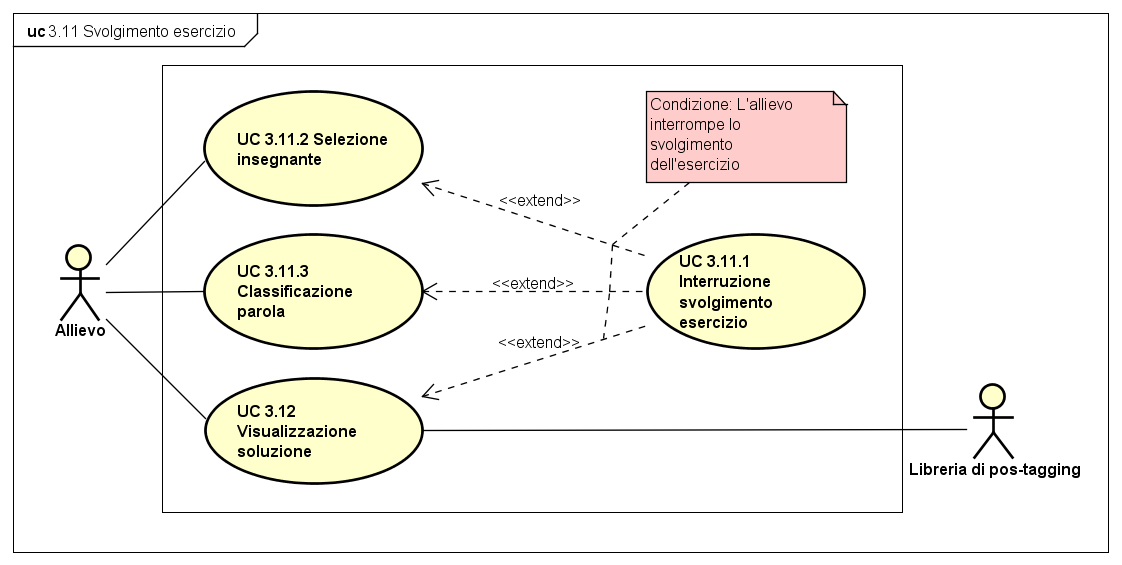
\includegraphics[width=17cm]{img/UC311.png} 
	\caption{Caso d'uso 3.11}\label{fig:311}
\end{figure}
\begin{itemize}
	\item[•]\textbf{Attori}: Allievo;
	\item[•]\textbf{Descrizione}: L'allievo può svolgere l'esercizio scegliendo le classi grammaticali per ciascuna parola da una apposita lista;
	\item[•]\textbf{Precondizione}: l'allievo ha selezionato un esercizio;
	\item[•]\textbf{Postcondizione}: l'allievo ha svolto un esercizio;
	\item[•]\textbf{Flusso degli eventi}:
	\begin{enumerate}
		\item Selezione esercizio;
		\item UC 3.11.2 - Selezione insegnante;
		\item UC 3.11.3 - Classificazione parola;
		\item UC 3.12 - Visualizzazione soluzione.
	\end{enumerate}
	\item[•]\textbf{Estensioni}:
	\begin{enumerate}
		\item UC 3.11.1 - Interruzione svolgimento esercizio.
	\end{enumerate}
\end{itemize}

\subsubsection{UC 3.11.1 - Interruzione svolgimento esercizio}
\begin{itemize}
	\item[•]\textbf{Attori}: Allievo;
	\item[•]\textbf{Descrizione}: l'allievo interrompe  l'esercizio, scartando i dati inseriti fino a quel momento, e ritorna nella sezione di visualizzazione elenco esercizi;
	\item[•]\textbf{Precondizione}: l'allievo inizia a svolgere un esercizio;
	\item[•]\textbf{Postcondizione}: l'allievo interrompe l'esercizio, torna nella sezione di visualizzazione elenco esercizi.
\end{itemize}

\subsubsection{UC 3.11.2 - Selezione insegnante}
\begin{itemize}
	\item[•]\textbf{Attori}: Allievo;
	\item[•]\textbf{Descrizione}: l'allievo seleziona l'insegnante da cui vuole ricevere la correzione dell'esercizio, se nessun insegnante ha predisposto quella frase verrà utilizzato il sistema di correzione automatico; %Quando è possibile l'insegnante preferito viene selezionato automaticamente;
	\item[•]\textbf{Precondizione}: l'allievo ha selezionato un esercizio;
	\item[•]\textbf{Postcondizione}: l'allievo seleziona l'insegnante dal quale vuole ricevere la correzione.
\end{itemize}

\subsubsection{UC 3.11.3 - Classificazione parola}
\begin{itemize}
	\item[•]\textbf{Attori}: Allievo;
	\item[•]\textbf{Descrizione}: l'allievo seleziona la classe grammaticale di una parola da una lista predefinita;
	\item[•]\textbf{Precondizione}: l'allievo sta svolgendo un esercizio;
	\item[•]\textbf{Postcondizione}: l'allievo seleziona la classe grammaticale di una parola.
\end{itemize}


\subsubsection{UC 3.12 - Visualizzazione soluzione}
\begin{figure}[H]
	\centering
	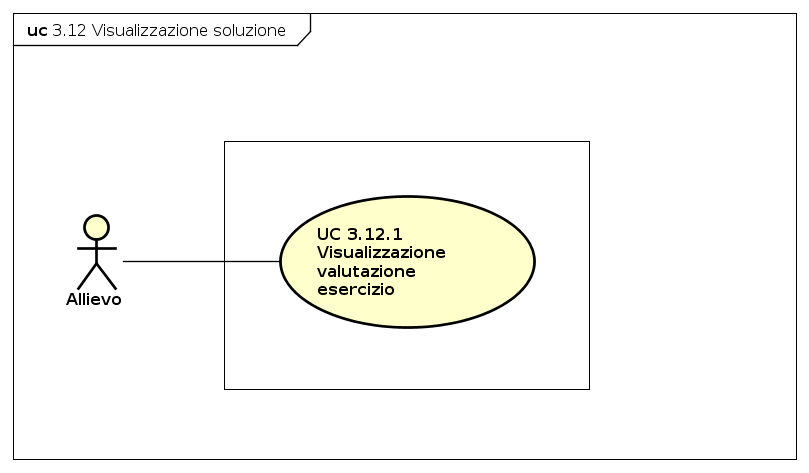
\includegraphics[width=17cm]{img/UC312.png} 
	\caption{Caso d'uso UC 3.12}\label{fig:312}
\end{figure}
\begin{itemize}
	\item[•]\textbf{Attori}: Allievo, Libreria di pos-tagging;
	\item[•]\textbf{Descrizione}: l'allievo visualizza la correzione secondo l'insegnante selezionato in precedenza. Se era stata inserita una frase libera la correzione viene eseguita dal sistema di correzione automatico;
	\item[•]\textbf{Precondizione}: l'allievo ha svolto un esercizio oppure ha inserito una frase libera;
	\item[•]\textbf{Postcondizione}: l'allievo visualizza la soluzione dell'esercizio;
	\item[•]\textbf{Flusso degli eventi}:
	\begin{enumerate}
		\item UC 3.12.1 - Visualizzazione valutazione esercizio.  
	\end{enumerate}
\end{itemize}


\subsubsection{UC 3.12.1 - Visualizzazione valutazione esercizio}   

\begin{itemize}
\item[•]\textbf{Attori}: Allievo;
\item[•]\textbf{Descrizione}: l'allievo riceve una valutazione in base al numero di parole classificate correttamente. Se sono presenti più soluzioni proposte dallo stesso insegnante viene presa la soluzione che porta alla valutazione più alta.
\item[•]\textbf{Precondizione}: l'allievo visualizza la soluzione dell'esercizio svolto;
\item[•]\textbf{Postcondizione}: l'allievo visualizza una valutazione sull'esercizio svolto.
\end{itemize}


